\subsection{Radiation Patterns: Antenna Adventures on Slopes vs. Flatlands!}

\begin{tcolorbox}[colback=gray!10, colframe=black, title=E9C14] 
How does the radiation pattern of a horizontally-polarized antenna mounted above a long slope compare with the same antenna mounted above flat ground?

\begin{enumerate}[label=\Alph*.]
    \item The main lobe takeoff angle increases in the downhill direction
    \item \textbf{The main lobe takeoff angle decreases in the downhill direction}
    \item The horizontal beamwidth decreases in the downhill direction
    \item The horizontal beamwidth increases in the uphill direction
\end{enumerate} \end{tcolorbox}

\subsubsection{Conceptual Background}

To understand the relationship between the radiation pattern of antennas and their mounting conditions, we first need to comprehend the nature of antenna radiation patterns. The radiation pattern of an antenna represents how it radiates electromagnetic energy into space. It is typically represented as a three-dimensional diagram indicating the strength of radiation emitted in various directions.

In this particular scenario, we focus on a horizontally-polarized antenna. Horizontally-polarized antennas radiate energy primarily in a plane perpendicular to the direction of the antenna's main axis. The takeoff angle refers to the angle at which the main lobe of the radiated energy leaves the antenna.

The two scenarios presented involve the antenna being mounted above flat ground and above a long slope. The main factor influencing the radiation pattern in these scenarios is the angle of the ground. A slope impacts the effective radiation angle due to its geometry.

\subsubsection{Analysis of Choices}

- \textbf{Choice A:}: The assertion that the main lobe takeoff angle increases in the downhill direction contradicts the behavior of antennas above sloped ground.
- \textbf{Choice B:}: This is the correct answer. When the slope is downhill, the effective height of the antenna's main lobe is lower, leading to a decrease in the takeoff angle in the downhill direction. 
- \textbf{Choice C:}: The horizontal beamwidth is not directly affected by the slope in this case, making this a misleading choice.
- \textbf{Choice D:}: Similarly, the horizontal beamwidth’s behavior given the slope is not applicable to the question context.

\subsubsection{Detailed Explanation with Diagrams}

Let's visualize this concept. Consider an antenna on a flat terrain and the same antenna on a slope as shown below:

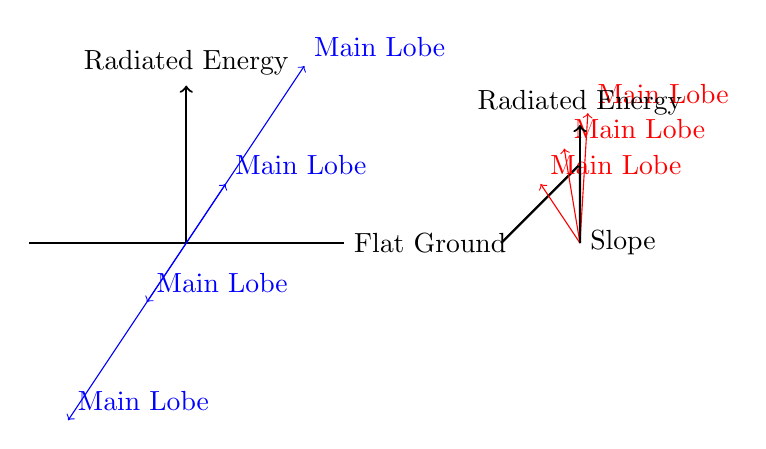
\begin{tikzpicture}[scale=1]
    \draw[thick] (-2,0) -- (2,0) node[right] {Flat Ground};
    \draw[thick,->] (0,0) -- (0,2) node[above] {Radiated Energy};
    \foreach \x in {-1.5, -0.5, 0.5, 1.5} {
        \draw[->, blue] (0,0) -- (\x,{1.5*\x}) node[above right] {Main Lobe};
    }
    \draw[thick] (4,0) -- (5, 1) -- (5,0) node[right] {Slope};
    \foreach \x in {4.5, 4.8, 5.1} {
        \draw[->, red] (5,0) -- ({\x},{1.5*\x - 6}) node[above right] {Main Lobe};
    }
    \draw[thick,->] (5,0) -- (5,1.5) node[above] {Radiated Energy};
\end{tikzpicture}

From the diagram, it can be seen that when the antenna is placed above a slope, the effective main lobe takeoff angle decreases in the downhill direction, confirming that the wave propagates with a lower angle compared to a flat ground installation.

Thus, a solid grasp of antenna radiation patterns and environmental impacts is crucial for successfully interpreting the question and selecting the correct answer.
